\section{Motivation}
\label{sec:motivation}
Das Rutherford-Streuexperiment, welches von Geiger und Mardsen durchgeführt
wurde, hat nach seiner Beendigung 1913 das Verständnis vom Aufbau des Atoms
fundamental verändert.
In diesem Versuch geht es darum die richtungsweisenden Ergebnisse,
in Teilen, nachzumessen und ihre Bedeutung nachzuvollziehen.

\section{Theorie}
\label{sec:theorie}
Die Wechselwirkung der $\ce{^4He}$-Kerne, bzw. \alphat, mit der Materie
erfolgt im Theoriemodell auf zwei Arten.

\subsection{\glname{Bethe-Bloch}{-Formel}}
Wenn die \alphat\:durch die Folie hindurchfliegen und mit den Elektronen
der Atomhüllen wechselwirken
ist der daraus resultierende Energieverlust durch die \glname{Bethe-Bloch}{-Formel} gegeben \cite{povh}:
\begin{equation}
  -\frac{\ud E}{\ud x} = -
  \frac{4 \mpi z^2 e^4 n}{m_e v^2 (4\mpi ε_0)^2}
  \ln\left(\frac{2 m_e v^2}{I}\right)
  \label{eqn:bethe-bloch} \\
\end{equation}
\begin{align*}
  z &= 2 \\
  v &= \text{Geschwindigkeit des \alphat s} \\
  I &\approx (\SI{10}{\electronvolt})\cdot Z \quad\text{Ionisationsenergie des Streuatoms} \\
  n &= \frac{Z \cdot ρ}{A \cdot u} \quad \text{Elektronendichte} \\
  ρ &= \text{Materialdichte}
\end{align*}

\subsection{\glname{Rutherford}{sche}-Streuformel}
Die zweite Möglichkeit ist die Streuung der \alphat\:an den Atomkernen.
Dieses wird durch die \glname{Rutherford}{sche}-Streuformel beschrieben
\begin{equation}
  \frac{\ud σ}{\ud Ω}(θ) = \frac{1}{(4\mpi ε_0)^2}
  \left(\frac{z Z e^2}{4 E_α}\right)^{\!\!2}
  \frac{1}{\sin^4 \left(\frac{θ}{2}\right)}
  \label{eqn:rutherford}
\end{equation}
$Z$ und $z$ sind die Kernladungszahlen der beteiligten Teilchen
und $E_α$ ist die mittlere Energie der \alphat.
$θ$ bezeichnet den Winkel zwischen dem Einfallweg und der Streustrecke des \alphat s.

\subsection{Wirkungsquerschnitt}
Im Zusammenklang mit Streuexperimenten muss auch auf den Wirkungsquerschnitt eingegangen werden.
Der differentielle Wirkungsquerschnitt $\sfrac{\udσ}{\udΩ}$ gibt die Anzahl der in das Raumelement $\udΩ$ gestreuten Teilchen an.
Der Wirkungsquerschnitt $σ$ folgt mit der Integration über alle Raumwinkelelemente,
typischerweise in Kugelkoordinaten,
\begin{equation}
    σ = \int \frac{\udσ}{\udΩ} \udΩ\:.
\end{equation}

\subsection{Zerfall von $\ce{^{241}Am}$}
Die Quelle der \alphat\:ist ein $\ce{^{241}Am}$-Strahler.
Der Anfang der Zerfallsreihe ist, nach \cite{zerfall},
\begin{equation}
  \ce{^{241}Am} \stackrel{α}{\to} \ce{^{237}Np} \stackrel{α}{\to} \ce{^{233}Pa} \stackrel{β^-}{\to} \ce{^{233}U} \stackrel{α}{\to} \ce{^{229}Th} \stackrel{α}{\to} \ce{^{225}Ra}\:.
\end{equation}
Die Halbwertszeiten der ersten Zerfallsschritte sind
\begin{align}
  \ce{^{241}Am}:& &τ = \SI{432.6(6)}{\year} \\
  \ce{^{237}Np}:& &τ = \SI{2.144(7)e6}{\year} \\
  \ce{^{233}Pa}:& &τ = \SI{26.975(13)}{\day} \\
  \ce{^{233}U}:& &τ = \SI{1.592(2)e5}{\year}
\end{align}
Es wird das \alphat~aus dem Zerfall $\ce{^{241}Am} \stackrel{α}{\to} \ce{^{237}Np}$ betrachtet,
aufgrund der Halbwertszeiten.
Die Energie der \alphat~beträgt $E_α = \SI{5485.56}{\kilo\electronvolt}$ \cite{zerfall}.

\subsection{Surface-Barrier Detektor}
\label{sec:SurfaceBarrierDetektor}
Ein Surface-Barrier Detekor ist ein Halbleiterdetektor. Ein einfallendes geladenes Teilchen
kann ein Elektron aus dem Valenzband so anregen, dass es in das Leitungsband springen kann.
Die zurückbleibende effektive positive Ladung wird als Loch bezeichnet.
Elektron und Loch werden durch ein angelegtes elektrisches Feld zu den gegenüberliegenden Elektroden gezogen.
Die Feinauflösung des Detektors kann durch ein Gitter aus einzelnen kleineren Detektoren
oder durch die Bewegung eines Detektors erhöht werden.

\subsection{Drehschieberpumpe}
Der Versuch wird im Vakuum durchgeführt, damit die Energieabgabe der \alphat~an die Luft minimiert werden kann.
Dadurch wird die Reichweite der $α$-Strahlung erhöht.

Das Vakuum wird mit einer Drehschieberpumpe erzeugt.
Diese hat zur Besonderheit, dass der Rotor exzentrisch gelagert ist,
wie es in Abbildung \ref{fig:drehschieberpumpe} zu sehen ist.
Damit der Schöpfraum immer in mindestens zwei Kammern unterteilt ist, sind
im Rotor zwei Stäbe eingefasst,
die entweder durch Trägheit oder eine Feder zum Rand gedrückt werden.
Der Schöpfraum wird über Ventile belüftet.

\begin{figure}[ht]
  \centering
  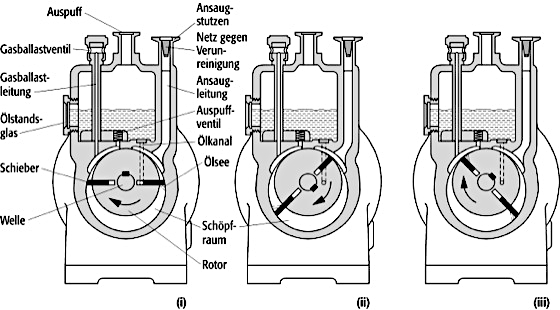
\includegraphics[width=0.8\textwidth]{images/drehschieberpumpe.jpg}
  \caption{Skizze einer Drehschieberpumpe zu verschiedenen Zeitpunkten \cite{drehschieberpumpe}.}
  \label{fig:drehschieberpumpe}
\end{figure}
\FloatBarrier

\subsection{Poisson-Verteilung}
Die verwendete Messmethode ist die Zählung der Teilchen mithilfe des Surface-Barrier Detektors.
Eine Zählung unterliegt immer der Poissonverteilung, die Standardabweichung dieser ist
\begin{align}
  σ_λ &= \sqrt{λ}
  \intertext{wenn $λ$ das Ergebnis ist. Es wird eine relativer Fehler von $\SI{3}{\percent}$ angestrebt.
  Dafür muss}
  \laplace_λ &= \frac{\sqrt{λ}}{λ} = \frac{1}{\sqrt{λ}} \stackrel{!}{=} \SI{3}{\percent} \\
  λ &= \frac{1}{(0.03)^2} = \num{1111.1}\:.
\end{align}
gelten.
